%%%--- Template for master thesis at SfS
%%%--- Modified template with more comments and examples -- SG, 11/06/09
%%%------
\documentclass[11pt,a4paper,twoside,openright]{report}
\usepackage[english]{ETHDAsfs}%--> ETHDASA + fancyhdr + ... "umlaute"
%  + sfs-hyper -> hyperref 

\usepackage{pdfpages}%%to include the confirmation of originality (plagiarism
\usepackage{amsbsy}%% for \boldsymbol and \pmb{.}
\usepackage{amssymb}%% calls  amsfonts...
\usepackage{graphicx}%-- für PostScript-Grafiken (besser als  psfig!)
%\usepackage[draft]{graphicx} % grafics shown as boxes --> faster compilation
%
\usepackage[longnamesfirst]{natbib}%was {sfsbib}%- Für  Literatur-Referenzen
%           ^^^^^^^^^^^^^^ 1) "Hampel, Ronchetti, ..,"  2) "Hampel et al"
% Engineers (and other funny people) want to see [1], [2] 
% ---> use 'numbers' : \usepackage[longnamesfirst,number]{natbib}
%
%
\usepackage{texab}%- 'tex Abkürzungen' /u/sfs/tex/tex/latex/texab.sty
        %%- z.B.  \R, \Z, \Q, \Nat für reelle, ganze, rationale, natürl. Zahlen;
        %%-       \N   (Normalvert.)  \W == Wahrscheinlichkeit .....
        %%-  \med, \var, \Cov, \....
        %%-  \abs{x} == |x|   und   \norm{y} ==  || y ||   (aber anständig)
%% NOTE: texab contains many useful definitions and "shortcuts". It is
%% worth to open the file and have a look at them. HOWEVER, some
%% definitions are a bit can lead to conflicts with other packages. You
%% might for example want to comment out the line defininf \IF as an
%% operator when working with the algorithmic package, or to comment out
%% the line defining a command \Cite with working with the Biblatex package  
\usepackage{amsmath}
%\usepackage{mathrsfs}% Raph Smith's Formal Script font --> provides \mathscr
\usepackage[utf8]{inputenc}% <<------- Unicode, *NOT* iso-latin1 !
\usepackage{ae}% A[lmost] E[uropean] Fonts
\usepackage{enumerate}% Fuer selbstdefinierte Nummerierungen
%--------
\usepackage{relsize}%-> \smaller (etc) used here
\usepackage{color} %% to allow coloring in code listings
\usepackage{listings}% Fuer R-code, C-code, ....  and settings for these:
\definecolor{Mygrey}{gray}{0.75}% for linenumbers only!
\definecolor{Cgrey}{gray}{0.4}% for comments
\lstloadlanguages{R}
%%--- first version of "listings of R"-style : ---------------------------
% %% using \smaller here: makes R code listings use a *small* font:
% \lstset{language=R,basicstyle=\smaller[2],commentstyle=\rmfamily\smaller,
%   showstringspaces=false,xleftmargin=4ex,
%   literate={<-}{{$\leftarrow$}}1 {~}{{$\sim$}}1}
% \lstset{escapeinside={(*}{*)}} % for (*\ref{ }*) inside lstlistings (Scode) 
%\newcommand{\lil}[1]{\lstinline|#1|}
%%--- newer version of "listings of R"-style : ---------------------------
\lstset{%% Help, e.g. --> https://en.wikibooks.org/wiki/LaTeX/Source_Code_Listings
language=R,
basicstyle=\ttfamily\scriptsize,%%- \small > \footnotesize > \scriptsize > \tiny
%commentstyle=\ttfamily\color{Cgrey},
commentstyle=\itshape\color{Cgrey},
numbers=left,
numberstyle=\ttfamily\color{Mygrey}\tiny,
stepnumber=1,
numbersep=5pt,
backgroundcolor=\color{white},
showspaces=false,
showstringspaces=false,
showtabs=false,
frame=single,
tabsize=2,
captionpos=b,
breaklines=true,
%breakatwhitespace=false,
keywordstyle={},
morekeywords={},
xleftmargin=4ex, 
literate={<-}{{$\leftarrow$}}1 {~}{{$\sim$}}1}
\lstset{escapeinside={(*}{*)}} % for (*\ref{ }*) inside lstlistings (Scode) 
%%----------------------------------------------------------------------------

%%------- Theoreme ---
\newtheorem{definition}{Definition}[subsection]
\newtheorem{lemma}[definition]{Lemma}
\newtheorem{theorem}[definition]{Theorem}
\newtheorem{Coro}[definition]{Corollary}
\theoremstyle{definition} 
\newtheorem{example}[definition]{Example}
\newtheorem*{note}{Note}
\newtheorem*{remark}{Remark}

\DeclareMathOperator*{\plim}{plim}
% \def\MR#1{\href{http://www.ams.org/mathscinet-getitem?mr=#1}{MR#1}}

% \newcommand{\Lecture}[3]{\marginpar{#3.#2.#1}}
% \newcommand{\Fu}{\mathcal{F}}
\newcommand{\aatop}[2]{\genfrac{}{}{0pt}{}{#1}{#2}}

%\renewcommand{\theequation}{\arabic{equation}}
\numberwithin{equation}{subsection}

%%%%%%%%%%%%%%%%%%%%%%%%%%%%%%%%%%%%%%%%%%%%%%%%%
%%% Path for your figures                      %%%
%%%%%%%%%%%%%%%%%%%%%%%%%%%%%%%%%%%%%%%%%%%%%%%%%
% Set the paths where all figures are taken from:
\graphicspath{{Pictures/}}

%%%%%%%%%%%%%%%%%%%%%%%%%%%%%%%%%%%%%%%%%%%%%%%%%
%%% Define your own commands here             %%%
%%%%%%%%%%%%%%%%%%%%%%%%%%%%%%%%%%%%%%%%%%%%%%%%%
\newcommand{\Bruch}[2]{{}^{#1}\!\!/\!_{#2}}
\renewcommand{\labelenumi}{\roman{enumi}.)}



\begin{document}
\bibliographystyle{chicago}% ---> Hampel,F., E.Ronchetti,... W.Stahel(1986) ...
 %was \bibliographystyle{sfsbib}\citationstyle{dcu} %OR DEFAULT : \citationstyle{agsm}

\pagenumbering{roman}%- roman numbering for first few pages

%%%%%%%%%%%%%%%%%%%%%%%%%%%%%%%%%%%%%%%%%%%%%%%%%
%%% Title page                                %%%
%%%%%%%%%%%%%%%%%%%%%%%%%%%%%%%%%%%%%%%%%%%%%%%%%
\period{Summer 2009}
\dasatype{Master Thesis}
\students{Student Muster}
\mainreaderprefix{Adviser:}
\mainreader{Prof.\ Dr.\ Sara van de Geer}
\alternatereaderprefix{Co-Adviser}
\alternatereader{Markus Kalisch}
\submissiondate{August 19th 2009}
\title{The title of my thesis \\ which should be split on \\ several lines
  if it is too long}

\maketitle%- Titelseite wird abgeschlossen
\cleardoublepage
 %%~~~~~~~~~~~~~~~~~~~~~~~~~~~~~~~~~~~~~~~~

%%%%%%%%%%%%%%%%%%%%%%%%%%%%%%%%%%%%%%%%%%%%%%%%%
%%% Insert here acknowledgements and abstract %%%
%%%%%%%%%%%%%%%%%%%%%%%%%%%%%%%%%%%%%%%%%%%%%%%%%
%% Dedication (optional)
\markright{}
\vspace*{\stretch{1}}
\begin{center}
    To some special person
\end{center}
\vspace*{\stretch{2}}

% Preface (optional)
\newpage
\markboth{Preface}{Preface}
\chapter*{Preface}

First words and acknowledgements.

XXX

Betreuung von Gregor

Ideen mit Meinshausen

Resourccen vom SFS

%%% Local Variables: 
%%% mode: latex
%%% TeX-master: "MasterThesisSfS"
%%% End: 


% Abstract should not be longer than one page.
\newpage
\markboth{Abstract}{Abstract}
\chapter*{Abstract}

%% Intro
Multispectral satellite imagery is used to model vegetation characteristics and development on a large scale in agriculture. As an example, satellite-derived Time Series (TS) of spectral indices like the Normalized Difference Vegetation Index (NDVI) are used to classify crops and to predict crop yield. 
%% Problem Illustration
Sometimes satellite measurements do not match the ground signal due to contamination by clouds and other atmospheric effects. Therefore, traditional approaches aim to filter out contaminated observations before extracting and subsequently interpolating the NDVI. After filtering, remaining contaminated observations and resulting data gaps are the two challenges for interpolation that we address in this thesis.
%% Our Setting
For this purpose, cereal crop yield maps from 2017-2021 of a farm in Switzerland with the corresponding Sentinel 2 satellite image TS published by the European Space Agency were examined. Contaminated observations were filtered with the provided Scene Classification Layer (SCL). 
%% NDVI itpl
We give a benchmark-supported review of different interpolation methods. Based on it, we found Smoothing Splines as a flexible non-parametric method and Double Logistic approximation as a parametric method with implicit shape assumptions to perform most favorably given the aforementioned challenges. In addition, we generalize an iterative technique which robustifies interpolation methods against outliers by reducing their weights. In most cases, this robustification successfully decreased the 50\% and 75\% quantiles of the absolute out-of-bag residuals. 
%% NDVI corr. 
Moreover, we present a general interpolation procedure that utilizes additional information to correct the target variable with an uncertainty estimate and then performs a weighted interpolation. In our setting, the target variable is the NDVI and as additional information we use the SCL, the observed NDVI and the spectral bands. Consequently, we no longer filter using the SCL, but weight observations according to their reliability. % The combination of different interpolation methods and correction models yields 28 interpolation strategies. % To choose the best one, we assume that, the better the interpolated NDVI TS models crop growth, the more suitable it is to predict crop yield. 
% {The resulting interpolation strategy uses Smoothing Splines and corrects the NDVI with uncertainty estimation through a simple linear model considering only of the observed NDVI and the associated SCL class.} 
Applying this procedure, the unexplained variance in crop yield estimations via the resulting NDVI TS decreased by~10.5\%. 
% Impact
Considering the success of the presented procedure with respect to NDVI TS, it appears promising for applications to other satellite-based TS given its cloud-correcting properties.

% %% Reproducibility  +  R-package
% Instructions and a codebase for reproducibility of the results, as well as an R package making the presented general interpolation procedure accessible to the user, are supplied. 



%%% Local Variables: 
%%% mode: latex
%%% TeX-master: "MasterThesisSfS"
%%% End: 


%%%%%%%%%%%%%%%%%%%%%%%%%%%%%%%%%%%%%%%%%%%%%%%%%
%%% Table of contents and list of figures and %%%   
%%% tables (no need to change this usually)   %%%
%%%%%%%%%%%%%%%%%%%%%%%%%%%%%%%%%%%%%%%%%%%%%%%%%
\newpage
\tableofcontents
\newpage
\listoffigures
\newpage
\listoftables

%% Notations and glossary (optional)
\cleardoublepage
\phantomsection
\addcontentsline{toc}{chapter}{\protect\numberline{}{Notation}}
\markboth{Notation}{Notation}
\chapter*{\vspace{-3.2cm} Notations}
\label{c:Notation}
\vspace{-0.6cm}
Since this thesis, despite its applied nauture, is located at the Mathematics Department, we adhere to the convention of speaking in the first person plural ``we''.\\
Moreover, only equations that are referenced elsewhere are equipped with a number.

\section*{Variables}\vspace{-0.2cm}
\renewcommand{\arraystretch}{1.3} % for non-dense tables
\begin{longtable}{p{0.12\linewidth} p{0.87\linewidth}}
$c$		& a (vector of) constant(s)\\
$\lambda \in \R$		& a scalar\\
$n\in \mathbb{N}$		& sample size\\
$i,j$		& indices in $\{1,\dots,n\}$\\
$n\in \R^n$		& time, usually in GDD\\
$w \in \R^n$		& a vector of weights for each location $x$\\
$y\in \R^n$		& response in 1-dim interpolation setting\\
$\hat y\in \R^n$		& estimate of $y$\\
$\bar y\in \R$		& sample mean of $y$\\
$r \in \R^n$		& residuals given by $y - \hat y$\\
$X\in\R^{n\times p}$ & the design matrix. Each row corresponds to one observation and each column to one covariate.\\
$X_{[:,j]}$ 	& the $j$-th column of $X$\\
$X_{[i,:]}$ 	& the $i$-th row of $X$
% $x\in \R^n$		& covariable in 1-dim interpolation setting
\end{longtable}

%%%%%%%%%%%%%%%%%%%%%%%%%%%
\section*{Abbreviations and Objects}\vspace{-0.2cm}
\begin{longtable}{p{0.12\linewidth} p{0.87\linewidth}}
NDVI	
		& Normalized Difference Vegetation Index \citep{rouseMonitoringVernalAdvancement1974}.\\

TS	
		& Time Series. \\
IM	
		& Interpolation Method. That is a simple\footnote{I.e., no combination of various methods.} method that interpolates data $(t_i,y_i)_{i = 1,\dots ,n}$ and yields a function $f(t)=y$, approximating the data. \\
IS	
		& Interpolation Strategy. This is the category of functions that map $(t_i,y_i)_{i=1,\dots,n}$ to a function $f(t)=y$, approximating the data. So a IS describes a strategy of how to arrive at an interpolation starting from the data $(t_i,y_i)_{i=1,\dots,n}$. For this, initial data may be corrected (cf. chapter~\ref{sec:corr}), (possible different) IMs (iteratively) used, weightings applied (cf. robustification in section~\ref{sec:loess_robustify}). Note, that strictly speaking every IM also is an IS. But usually we expect an IS to involve a more `complex' procedure. \\
S2	
		& Sentinel 2 satellites. Two multi-spectral image satellites deployed by the European Space Agency. \\
SCL	
		& Scene Classification Layer provided by the European Space Agency that gives an estimation of the land cover class of each pixel. It indicates what one can expect at a pixel at a sampled time. For an overview, see table~\ref{tab:satelite/scl_classes}\\
Pixel	
		& A pixel originates of an image pixel and describes a square of 10 x 10 meters in the field that coincides with the resolution (and location) of the Sentinel-2 pixels. Such pixels are illustrated in figure~\ref{fig:satelite/witzwil_2021_P112_yield_cropped.png}. Additional information like yield is also attached.\\

$P_t$	
		& the observed data (weather and spectral bands) at time $t$ and the location of one pixel. \\

$P$	
		& a pixel. We see it as a collection of all the observations at the specified location within one season. More formally, $P := \left\{P_t | t\text{ is a valid sample time within a defined season}\right\}$\\


$P^{SCL45}$	
		& is similar to $P$ but we only consider observations that belong to the classes 4 and 5. This is used done to get a subset of observations which are less contaminated by clouds and shadows.\\

DAS	
		& Days After Sowing\\

GDD	
		& Growing Degree Days -- cumulative sum of ``$\max(0, \text{temperature}-\text{threshold})$''\\

YPE 	
		& (Relative) Yiepld Prediction Error. See Definition~\ref{def:YPE}\\

OOB 	
		& Out Of the Box. Describes the procedure of  estimating the value for a point by a model that has not seen this point before (see section~\ref{sec:OOB_LOOCV}).\\

LOOCV 	
		& Leave One Out Cross Validation. Describes the procedure of estimating the value for a point by a model that has seen all the points except the current one (see section~\ref{sec:OOB_LOOCV}).
\end{longtable} 

\section*{Statistical Models}\vspace{-0.2cm}
\begin{longtable}{p{0.12\linewidth} p{0.87\linewidth}}
	DL
		& Double Logistic (see section~\ref{sec:double_logistic})\\
	FS
		& Fourier Series (see section~\ref{sec:fourier_approx})\\
	NW
		& Nadaraya-Watson (see section~\ref{sec:Kernel})\\
	UK
		& Universal Kriging (see section~\ref{sec:Kriging})\\
	SG
		& Savitzky-Golay Filter (see section~\ref{sec:Savitzky-Golay})\\
	LOESS
		& Locally Weighted Regression (see section~\ref{sec:loess})\\
	BS
		& B-splines (see section~\ref{sec:B})\\
	SS
		& Smoothing Splines (see section~\ref{sec:Natural_SS})\\
	OLS
		& Ordinary Least Squares (see section~\ref{sec:corr_model_OLS})\\
	OLS\textsuperscript{SCL}
		& OLS using only the observed NDVI and SCL classes (as factor variables)\\
	OLS\textsuperscript{all}
		& OLS using the covarietes OLS\textsuperscript{SCL} uses and the spectral bands\\
	LASSO
		& Least Absolute Shrinkage and Selection Operator (see section~\ref{sec:corr_model_LASSO})\\
	GAM
		& General Additive Model (see section~\ref{sec:corr_model_GAM})\\
	RF
		& Random Forest (see section~\ref{sec:corr_model_RF})\\
	MARS
		& Multivariate Adaptive Regression Splines (see section~\ref{sec:corr_model_MARS})\\
\end{longtable} \renewcommand{\arraystretch}{1}

% \bigskip











%%% Local Variables: 
%%% mode: latex
%%% TeX-master: "MasterThesisSfS"
%%% End: 


\cleardoublepage
\pagenumbering{arabic}%--- switch back to standard numbering 


%%%%%%%%%%%%%%%%%%%%%%%%%%%%%%%%%%%%%%%%%%%%%%%%%
%%% Your text... Either write here directly,  %%%
%%% or even better: write in separate files   %%%
%%% that you just have to include here.       %%% 
%%%%%%%%%%%%%%%%%%%%%%%%%%%%%%%%%%%%%%%%%%%%%%%%%
\chapter{Introduction}

Remote sensing aims to measure target variables efficiently from a distance. 
% stakeholders + applications  
Large scale monitoring of forest and agricultural vegetation dynamics is of great interest to authorities, insurance companies and research. Examples include crop classification for subsidizing farmers \citep{henitsSentinel2EnablesNationwide2022} and the creation of crop models for estimating crop yields or nitrogen concentrations \citep{couraultSTICSCropModel2021,perichCropNitrogenRetrieval2021}. 
% Season Start (start of spring) (community name: land surface plant phenology)
For this, freely distributed multi-spectral satellite imagery from the  Sentinel-2 (S2) satellites are examined \citep{esaSentinel22022}.
% NDVI
In order to transform the high dimensional satellite images into easily interpretable metrics, spectral indices such as the Normalized Difference Vegetation Index (NDVI) are used \citep{rouseMonitoringVernalAdvancement1974}. The NDVI serves as a proxy for photosynthetic activity \citep{gamonRelationshipsNDVICanopy1995a}, and thus the corresponding {NDVI Time Series ({TS})} reflects the vegetation development. 
% S2 issues (clouds ...)
The quality of a satellite image, however, depends on atmospheric conditions. Thus, in case of a dense cloud cover, the information content derived from the NDVI is impaired. Therefore, \cite{esaEuropeanSpaceAgency2022} also provides a Scene Classification Layer (SCL), which provides additional metadata about what is observed (e.g., shadows, clouds, vegetation, etc.) . So when extracting the NDVI {TS} from the Sentinel 2 satellite imagery {TS}, we can filter out the contaminated observations using the SCL classification. However, due to this filtration it may occur that we have no observations for several weeks, especially in winter. It is also possible that some observations are wrongly classified by the SCL (e.g., as vegetation) and thus result in an outlier in the NDVI TS. Consequently, the main challenge is to interpolate an NDVI {TS}, which can contain large data gaps and outliers. 

% state-of-the-art
Currently, there are several approaches to address these issues. One is to look at the observed evolution of the canopy coverage and assume its bell shape for the NDVI {TS} given the strong correlation between NDVI and photosynthetic activity. Approaches to model this include a \nth{2} order Fourier approximation \citep{stockliEuropeanPlantPhenology2004} or a Double Logistic function \citep{beckImprovedMonitoringVegetation2006}.
On the other hand, assumptions are made about more abstract properties of the curve, such as smoothness. We divide these into local and global approaches. Nadaraya-Watson \citep{strbacEstimationEvapotrasnpirationUrban2017}, Savitzky-Golay Filter \citep{chenSimpleMethodReconstructing2004a} and Locally Reweighed Regression \citep{omoriAssessmentPaddyFields2021} use a sliding window to interpolate the {TS} stepwise. Global methods like B-Splines \citep{gurungPredictingEnhancedVegetation2009} and Smoothing Splines \citep{caiPerformanceSmoothingMethods2017} reduce the squares of all residuals simultaneously, and Universal Kriging fits a Gaussian process to the data \citep{chandolaScalableTimeSeries2010}.
% SS defined in \cite{cravenSmoothingNoisyData1978}

\pagebreak
The research questions pursued in this thesis are:
\begin{Nenumerate}
    \item Which {{IM}}s are used in the context of NDVI, and what are their advantages and disadvantages?
    \item How may contaminated data be dealt with?
    \item How do data gaps affect interpolation?
    \item How to deal with data gaps?
    \item How can we recognize a good interpolation of the NDVI?
\end{Nenumerate}
\bigskip



% our contribution + roadmap:
In this thesis, we will discuss the strengths and weaknesses of Interpolation Methods ({{IM}}s) and evaluate them with respect to NDVI interpolation. For this purpose, we use the Sentinel 2 satellite image {TS} and crop yield maps of different fields of different cereal species on a farm in Witzwil, Switzerland over the years 2017-2021. After presenting the available data, illustrating challenges and defining different concepts in chapter~\ref{sec:data_methods} (\nameref{sec:data_methods}), we turn to the two main blocks of this thesis. One covers the study of IMs and the other presents a general procedure of correcting (NDVI) TS with uncertainty estimation by utilizing additional information.
On the first block, in chapter~\ref{sec:itpl} (\nameref{sec:itpl}) we examine parametric and non-parametric {{IM}}s and discuss their strengths and weaknesses (question i.). We generalize and test an iterative technique that makes IMs more robust to outliers by weighting them less (question ii.). To evaluate IMs, we present an approach that uses out-of-bag residuals (question v.). In section~\ref{sec:discussion_itpl_data_gaps} (\nameref{sec:discussion_itpl_data_gaps}), we discuss how different {{IM}}s respond to data gaps (question iii.), and in section~\ref{sec:itpl_preselection} (\nameref{sec:itpl_preselection}) we preselect {{IM}}s. This preselection, we evaluate in the results section~\ref{sec:results_itpl} (\nameref{sec:results_itpl}) and select two candidates from the {{IM}}s in section~\ref{sec:itpl_candiate_selection} (\nameref{sec:itpl_candiate_selection}).
For the second block, we correct possibly contaminated data with statistical models in chapter~\ref{sec:corr} (\nameref{sec:corr}) (question ii.) and utilize previously ignored observations, which we hope will further reduce data gaps (question iv.). Thus, we no longer filter the observations a priori via the SCL, but instead correct the observed NDVI and weight the observations via estimated uncertainties. By combining different statistical models and IMs, we obtain 28 Interpolation Strategies ({{ISs}}). We compare those with a vegetation-oriented quality measure (question v.) and describe the results in section~\ref{sec:results_ndvi_corr} (\nameref{sec:results_ndvi_corr}). Based on these results, in section~\ref{sec:discussion_corr} (\nameref{sec:discussion_corr}) we argue what the best {{IS}} is. In addition, we justify why our NDVI correction can be understood as unsupervised learning and why we relied only on satellite imagery and not on meteorological data for the NDVI correction.
Our conclusions of this thesis, recommendations, as well as an outlook on future work is given in chapter~\ref{sec:Conclusion} (\nameref{sec:Conclusion}). 


% und Definieren verschiedene Konzepte. Darunter eine transformation der Zeitachse, welche datenlücken im Winter zusammenschrumpfen lässt (Frage iv.). 




%smoothing:   ``Similarly, smoothing the {TS} of satellite data is helpful to address inconsistency in observation frequency and timing due to clouds and other sensor artefacts \cite{skakunWinterWheatYield2019}''


%%% Local Variables: 
%%% mode: latex
%%% TeX-master: "MasterThesisSfS"
%%% End: 

\chapter{First Chapter}

\section{To include a picture}
\begin{figure}[hbt!]%--- Picture 'H'ere, 'B'ottom or 'T'op; '!' Try to
  %impose your will to LaTeX
  \epsfCfile{.85}{geys-2kern} %<< no file extension
  %%         --- .85 stands for 85% of text width
  \caption[Geyser data: binned histogram, Silverman's and another
    kernel]%<<-- Legend for the list of figures at the beginning of you thesis
  {Old Faithful Geyser eruption lengths, $n=272$; binned data and two
    (Gaussian) kernel density estimates ($\times 10$) with $h=h^*= .3348$
    and $h= .1$ (dotted).}% legend displayed below the graph.
  \label{fig:geys1}
\end{figure}

Or also with \texttt{includegraphics}:
\begin{figure}[hbt!]%--- Picture 'H'ere, 'B'ottom or 'T'op; '!' Try to
  %impose your will to LaTeX
  \centering
  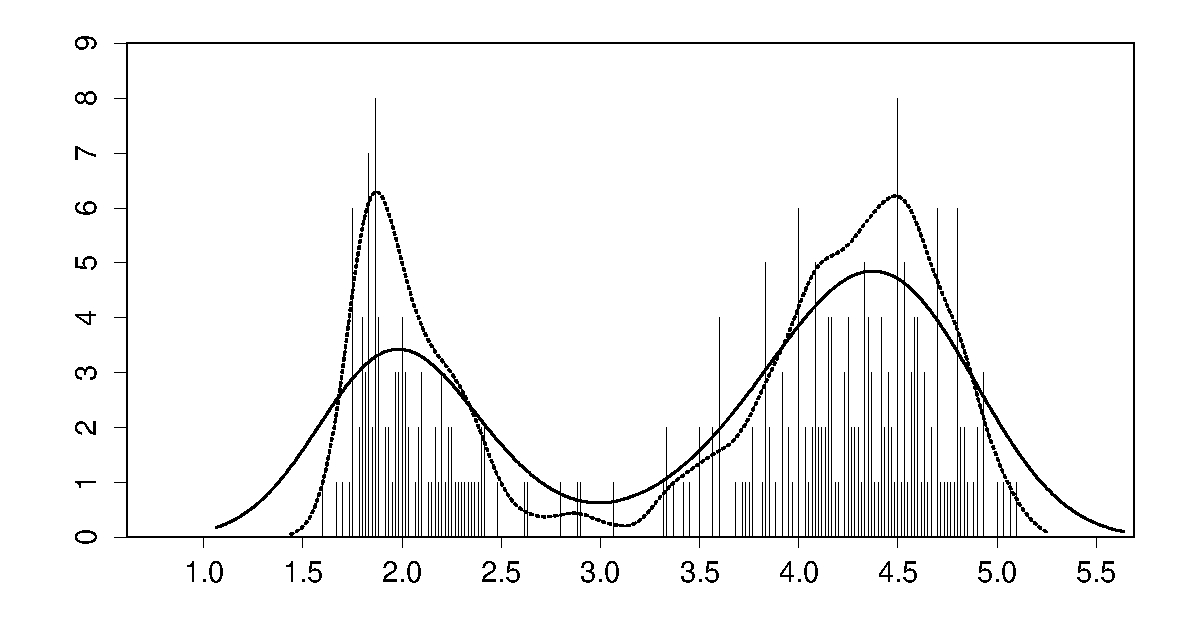
\includegraphics[width=.5\textwidth]{template-files/geys-2kern} %<< no file extension
  %%         --- .5\textwidth stands for 50% of text width
  \caption[Geyser data: binned histogram, Silverman's and another
    kernel]%<<-- Legend for the list of figures at the beginning of you thesis
  {Old Faithful Geyser eruption lengths, $n=272$; binned data and two
    (Gaussian) kernel density estimates ($\times 10$) with $h=h^*= .3348$
    and $h= .1$ (dotted).}% legend displayed below the graph.
  \label{fig:geys2}
\end{figure}

\section{To make a proof}
\begin{proof}
  $1 + 1 = 2$
\end{proof}

\section{To include \Rp code}
See information in Appendix~\ref{app:complement}.


\section{Other information}
Put a text between quotes: make sure to use nice quotes, such as `quote'.

Cite an article or book you refer shortly here, and then listed in the bibliography: \cite{ReferenceKey}.
%%--> in file   myReferences.bib  (same directory)
Or mention that \citeauthor{HamF85} (a person) or \citeauthor{StaWW91} (two
persons) have already done quite a bit work.

Referencing a different part of your work: please refer to Appendix~\ref{app:complement}.


%%% Local Variables: 
%%% mode: latex
%%% TeX-master: "MasterThesisSfS"
%%% End: 

%%\include{Chapter...}
\chapter{Summary}
\label{s:Summary}

Summarize the presented work. Why is it useful to the research field or institute?


\section{Future Work}
\label{ss:FutureWork}

Possible ways to extend the work.


%%% Local Variables: 
%%% mode: latex
%%% TeX-master: "MasterThesisSfS"
%%% End: 
 

%%%%%%%%%%%%%%%%%%%%%%%%%%%%%%%%%%%%%%%%%%%%%%%%%
%%% Bibliography                              %%%
%%%%%%%%%%%%%%%%%%%%%%%%%%%%%%%%%%%%%%%%%%%%%%%%%
\addtocontents{toc}{\vspace{.5\baselineskip}}
\cleardoublepage
\phantomsection
\addcontentsline{toc}{chapter}{\protect\numberline{}{Bibliography}}
\bibliography{myReferences}
%% All books from our library (SfS) are already in a BiBTeX file
%% 'Assbib.bib' (included here as well), using
% \bibliography{myReferences,Assbib}
% ---------------------------------- instead of the above



%%%%%%%%%%%%%%%%%%%%%%%%%%%%%%%%%%%%%%%%%%%%%%%%% 
%%% Appendices (if needed, e.g. for R code)   %%%
%%%%%%%%%%%%%%%%%%%%%%%%%%%%%%%%%%%%%%%%%%%%%%%%%
\addtocontents{toc}{\vspace{.5\baselineskip}}
\appendix
\chapter{Complementary information}
\label{app:complement}

Additional material. For example long mathematical derivations could be
given in the appendix. Or you could include part of your code that is
needed in printed form. You can add several Appendices to your thesis (as
you can include several chapters in the main part of your work).

\section{Including \Rp code with verbatim}
A simple (rather too simple, see~\ref{App:listings}) way to include code or
  {\it R} output is to use
\texttt{verbatim}. It just prints the text however it is (including all
spaces, ``strange'' symbols,...) in a slightly different font.
\begin{verbatim}
## loading packages
library(RBGL)
library(Rgraphviz)
library(boot)

## global variables
X_MAX <- 150

   This allows me to put as many s  p a   c es   as I want.
I can also use \ and ` and & and all the rest that is usually only 
accepted in the math mode.

I can also make as 
                  many 
             line 
    breaks as 
I want... and
             where I want. 
\end{verbatim}

But really recommended,  much better is the following:

\section{Including \Rp code with the \emph{listings} package}\label{App:listings}
However, it is much nicer to use the \emph{listings} package to include \Rp
code in your report. It allows you to number the lines, color the comments
differently than the code, and so on.
All the following is produced by simply writing
\verb! \lstinputlisting{figures/template-files/picture.R} !  in your \LaTeX\ ``code'':

\lstinputlisting{figures/template-files/picture.R}

or \verb!\lstinputlisting{/u/maechler/R/Pkgs/sfsmisc/R/misc/ellipse.R}! :

\lstinputlisting{misc/ellipse.R}% was /u/maechler/R/Pkgs/sfsmisc/R/misc/ellipse.R

\section{Using \texttt{Sweave} (or \texttt{knitr}) to include \Rp code (and more) in your report}
The easiest (and most elegant) way to include \Rp code and its output (and
have all your figures up to date with your report) is to use Sweave---or the
\href{https://cran.R-project.org/package=knitr}{\texttt{knitr}} R package with even more possibilities.
% You can find an introduction Sweave in \texttt{/u/sfs/StatSoftDoc/Sweave/Sweave-tutorial.pdf}.

Search the web to find lots of intro material on how to use Sweave or
\href{https://en.wikipedia.org/wiki/Knitr}{knitr (on Wikipedia)}.

%%% Local Variables: 
%%% mode: latex
%%% TeX-master: "MasterThesisSfS"
%%% End: 

\chapter{Yet another appendix....}

\section{Description}
\begin{description}
\item[Something] details.
\item[Something else] other definition.
\end{description}

\section{Tables}
Refer to Table~\ref{tab:example} to see a left justified table with caption
on top.

\begin{table}[ht]
\centering
\caption[Test results]{\label{tab:example}Results.}
\begin{tabular}{ll}
\hline
\textbf{Student} & \textbf{Grade}\\
\hline
Marie  & $6$\\
Alain  & $5.5$\\
Josette  & $4.5$\\
Pierre  & $5$\\
\hline
\end{tabular}
\end{table}

%%% Local Variables: 
%%% mode: latex
%%% TeX-master: "MasterThesisSfS"
%%% End: 

\chapter{2nd Appendix: More sophisticated R code listing} \label{appendix-more-R}

Chapter-wise listing of parts of R code, using
\begin{itemize}
\item \texttt{firstline=n1}
\item \texttt{lastline=n2}
\item \texttt{title=<text>}
\end{itemize}
e.g., for the first example below
\begin{verbatim}
\lstinputlisting[firstline=1,lastline=32,
                 title= \texttt{read\_irwls\_fn.R}]{../RCode/read_irwls_fn.R}
\end{verbatim}

% \section{Chapter 2} \label{app 2}

% \lstinputlisting[firstline=1,lastline=77,
% title=\texttt{analytic\_efficiency.R}]{../RCode/analytic_efficiency.R}
% %\lstinputlisting[firstline=,lastline=]{../RCode/???.R}

\bigskip% or even  \clearpage

%-----------------------------------------------------------------------------------------
\section{Chapter 5} \label{app 5}

% \lstinputlisting[firstline=1,lastline=71,
%                  title=\texttt{loss-fn\_rotated.R}]{../RCode/loss-fn_rotated.R}
\lstinputlisting[firstline=1,lastline=32,
                 title= \texttt{read\_irwls\_fn.R}]{ellipse.R}

\medskip
                 
\lstinputlisting[firstline=1,lastline=45,
                 title=\texttt{plot.psi.R}]{ellipse.R}
%\lstinputlisting[firstline=,lastline=]{../RCode/???.R}
%\lstinputlisting[firstline=,lastline=]{../RCode/???.R}

% \clearpage
%-----------------------------------------------------------------------------------------
% \section{Chapter 7} \label{app 7}

% \lstinputlisting[firstline=1,lastline=35,
%                  title= \texttt{stat.test} from \texttt{lmrob2-fn.R}]{../RCode/lmrob2-fn.R}
% \lstinputlisting[firstline=41,lastline=194,
%                  title=\texttt{M.optimal.ms} from \texttt{lmrob2-fn.R}]{../RCode/lmrob2-fn.R}
%\lstinputlisting[firstline=,lastline=]{../RCode/???.R}
%-----------------------------------------------------------------------------------------

%%% Local Variables:
%%% mode: latex
%%% TeX-master: "MasterThesisSfS"
%%% End:



%% Epilogue (optional)
\addtocontents{toc}{\vspace{.5\baselineskip}}
\cleardoublepage
\phantomsection
\addcontentsline{toc}{chapter}{\protect\numberline{}{Epilogue}}
\markboth{Epilogue}{Epilogue}
\chapter*{Epilogue}
\label{s:Epilogue}

A few final words.



%%% Local Variables: 
%%% mode: latex
%%% TeX-master: "MasterThesisSfS"
%%% End: 



%%%%%%%%%%%%%%%%%%%%%%%%%%%%%%%%%%%%%%%%%%%%%%%%%% 
%%% Declaration of originality (Do not remove!)%%%
%%%%%%%%%%%%%%%%%%%%%%%%%%%%%%%%%%%%%%%%%%%%%%%%%%
%% Instructions:
%% -------------
%% fill in the empty document confirmation-originality.pdf electronically
%% print it out and sign it
%% scan it in again and save the scan in this directory with name
%% confirmation-originality-scan.pdf 
%%
%% General info on plagiarism:
%% https://www.ethz.ch/students/en/studies/performance-assessments/plagiarism.html 
\cleardoublepage
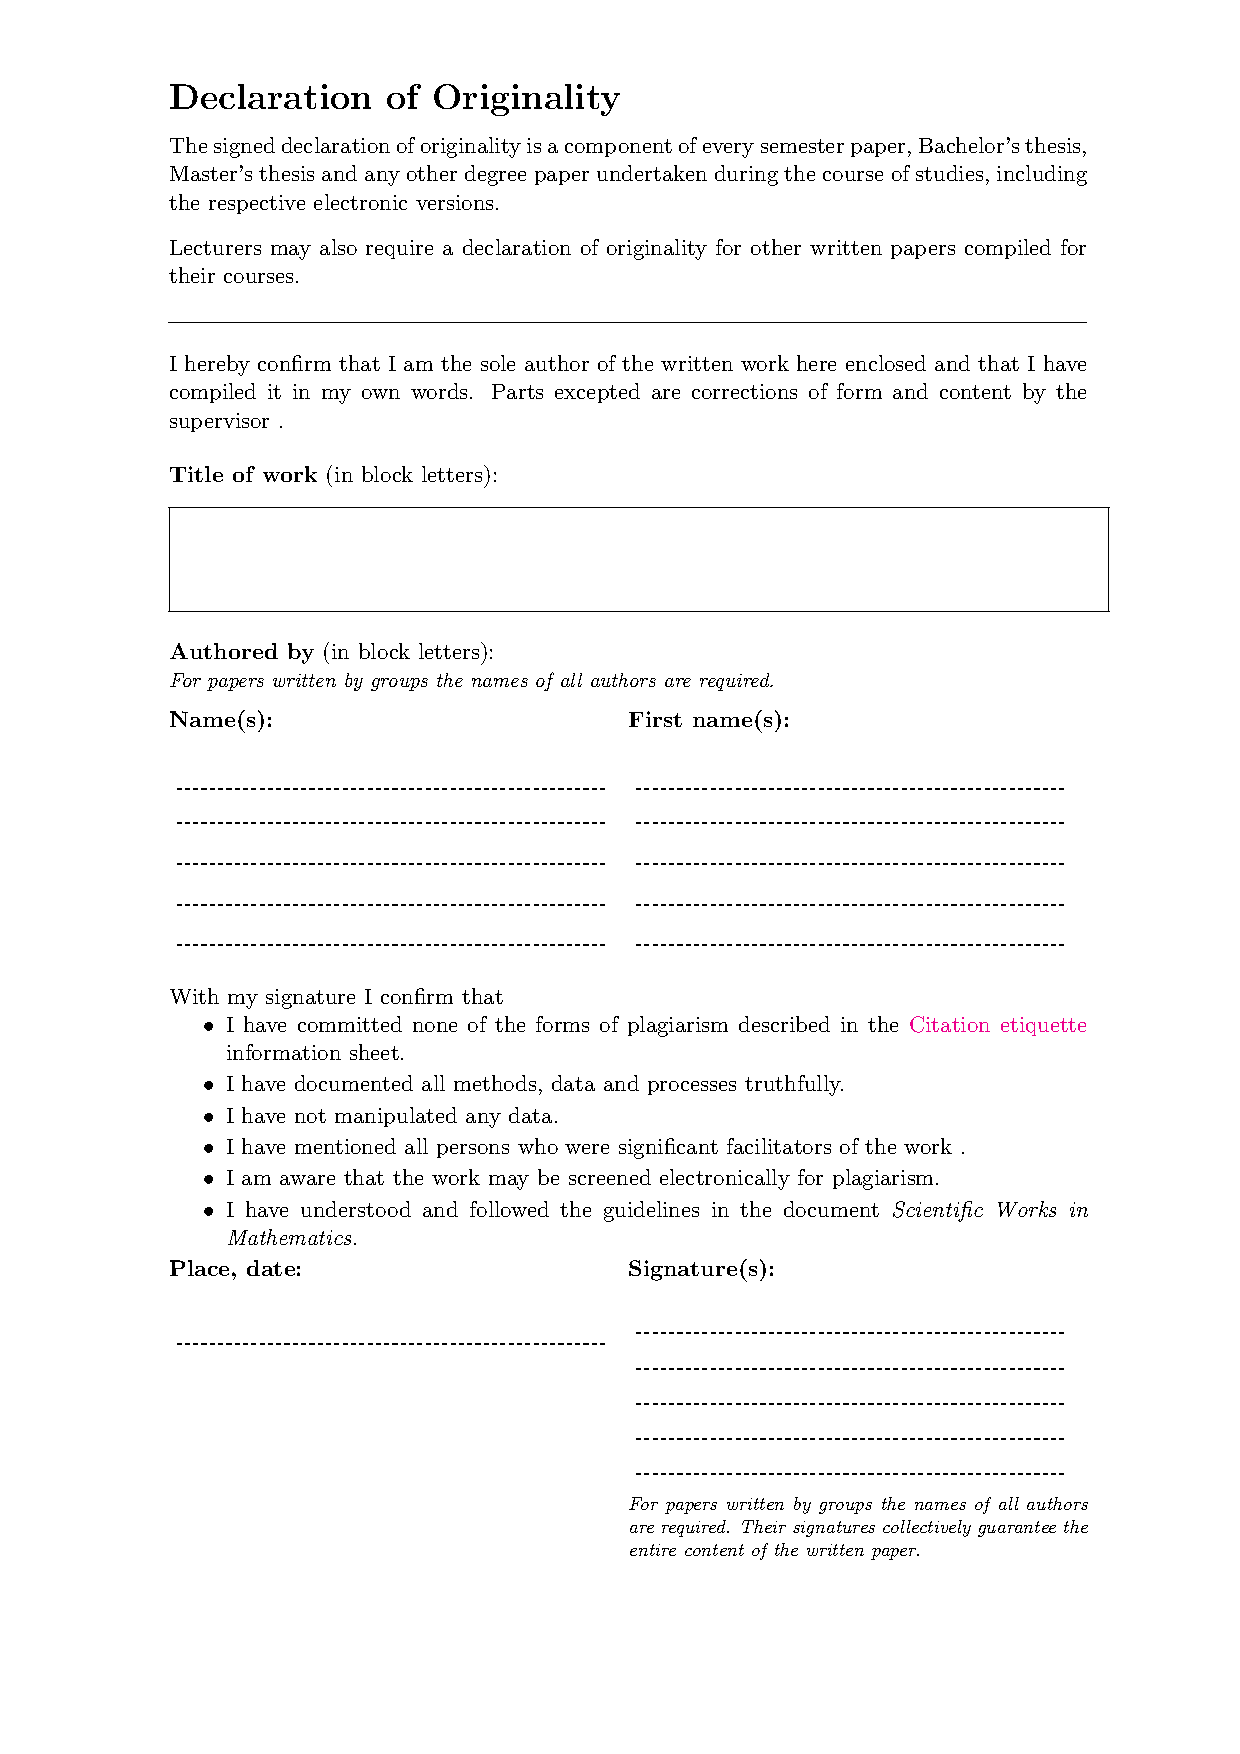
\includepdf[pages={-}, frame=true,scale=1]{confirmation-originality.pdf}
\end{document}

%%% Local Variables:
%%% mode: latex
%%% TeX-master: "MasterThesisSfS"
%%% End:
